\begin{appendices}
	\chapter{}
	\begin{figure}[H]
		\center{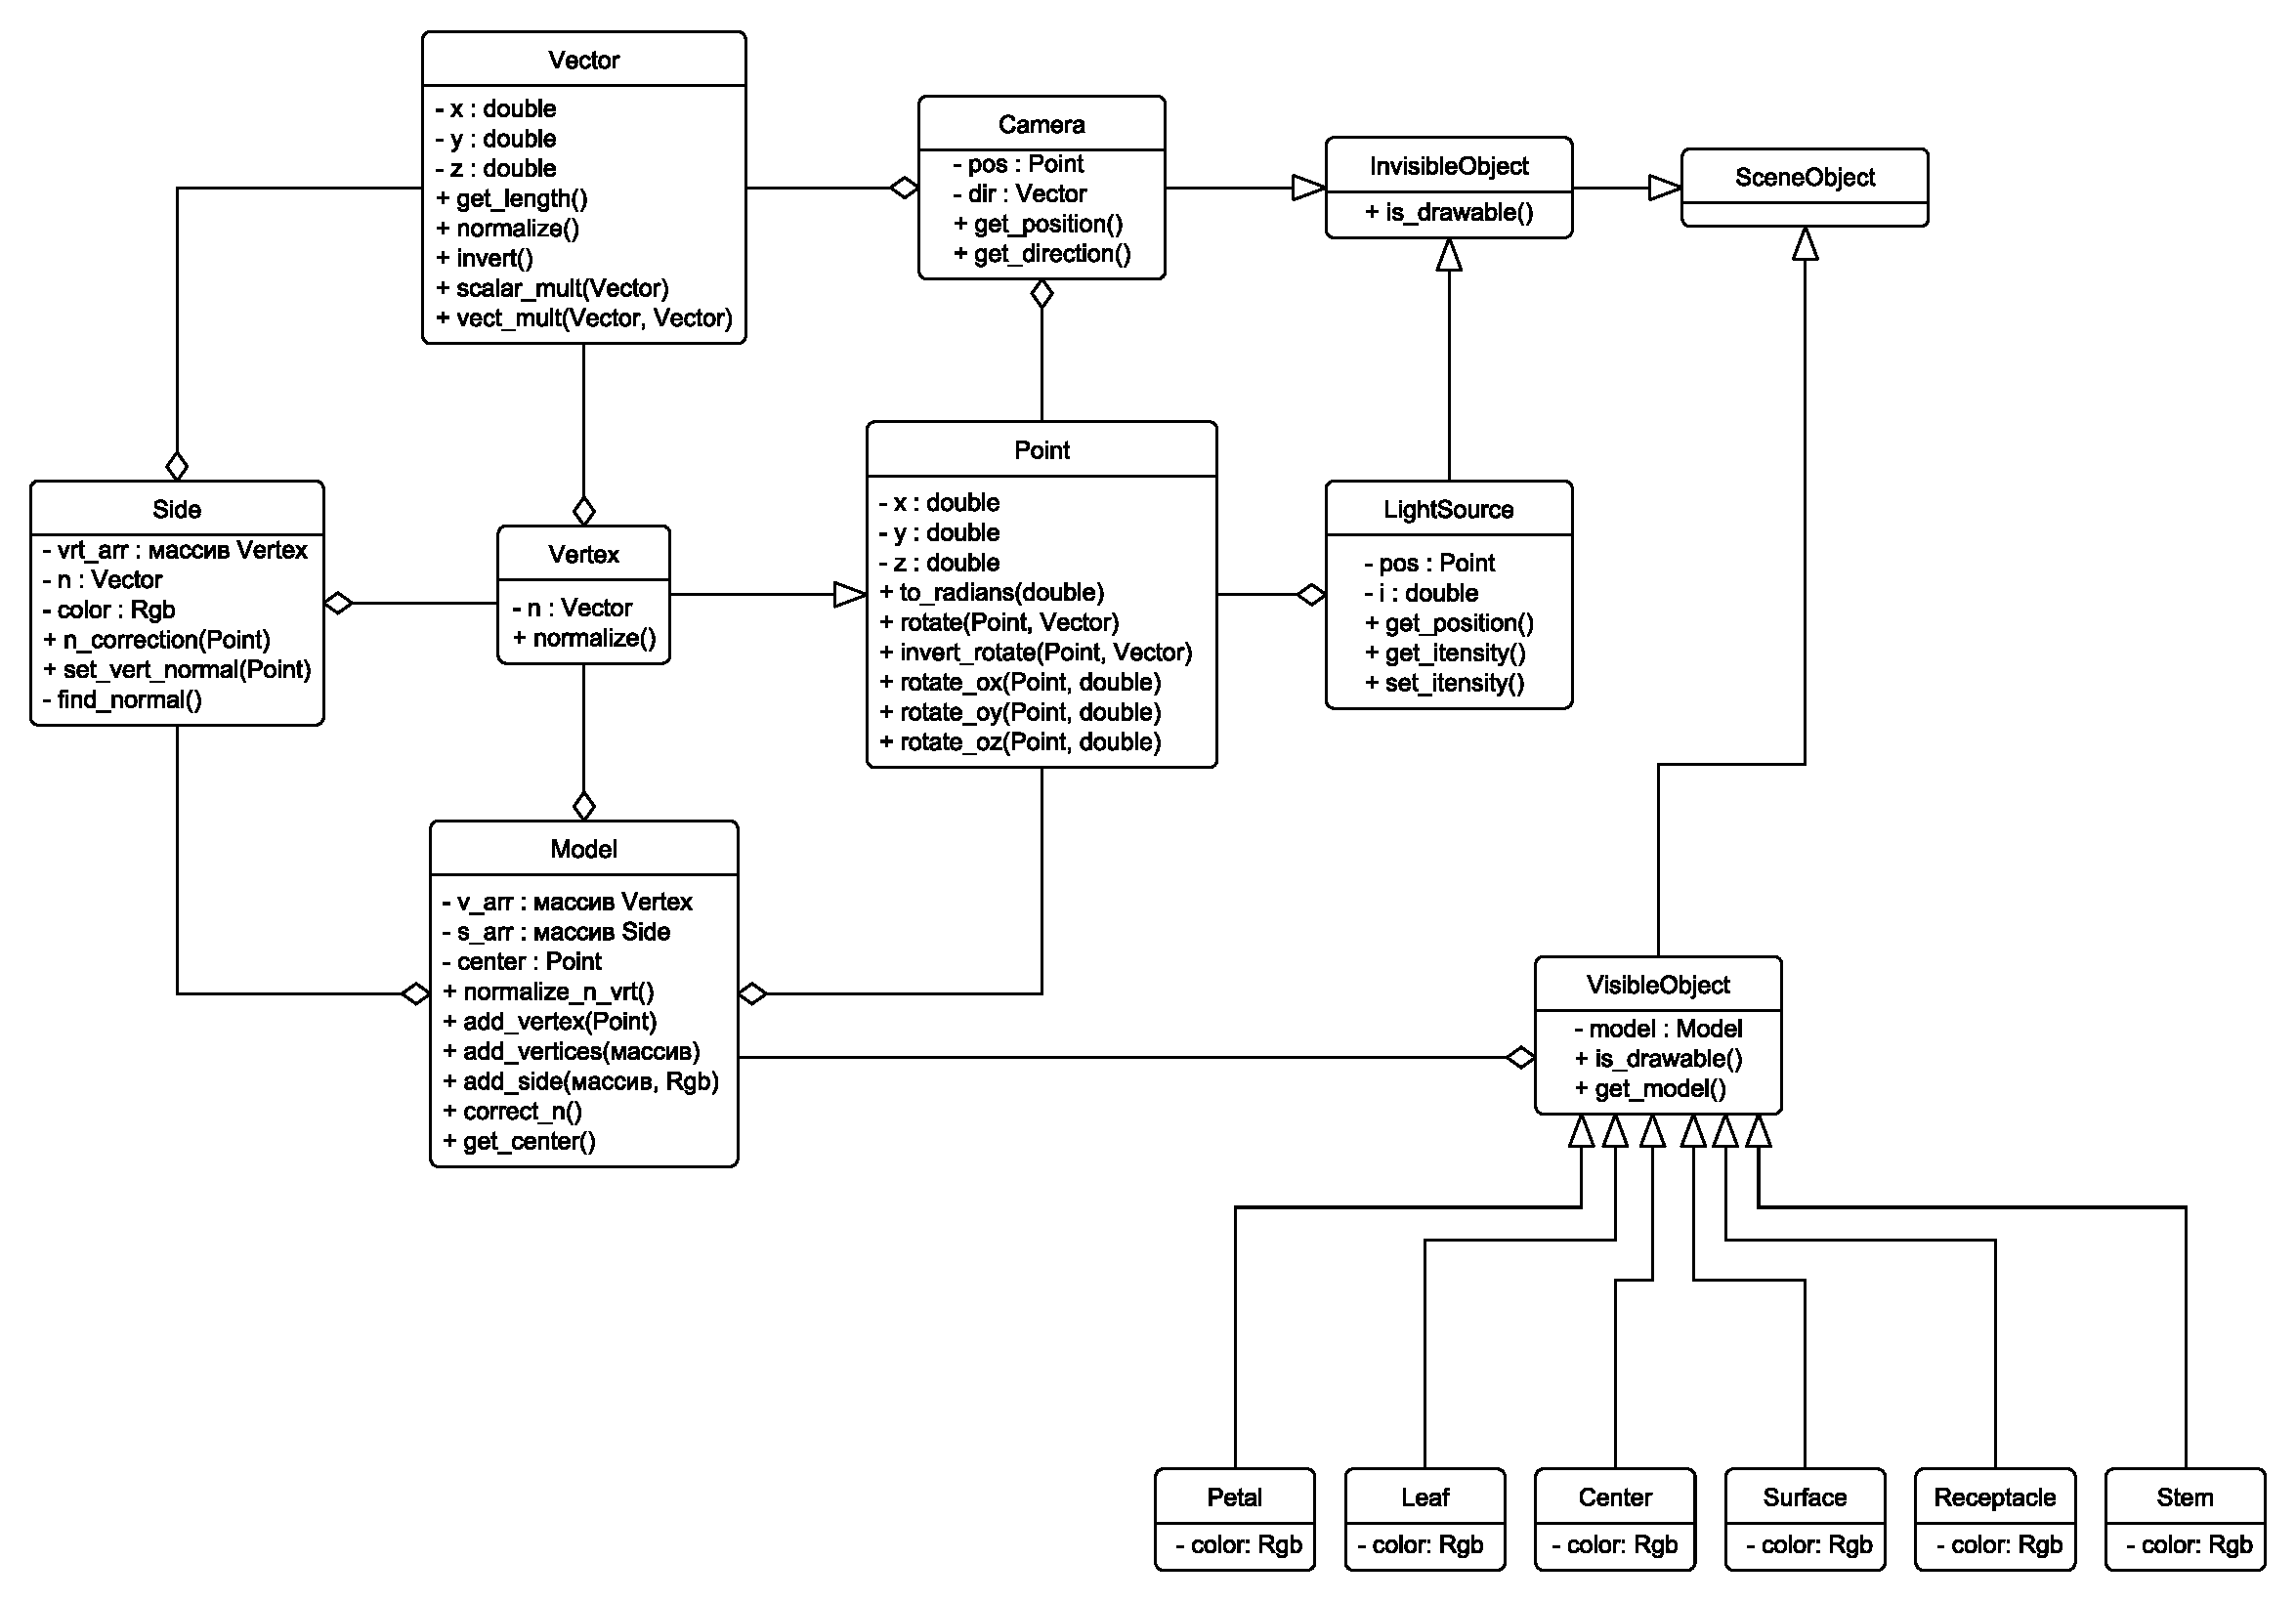
\includegraphics[angle=90,width=0.9\textwidth]{inc/img/uml}}
		\caption{Схема взаимодействия основных объектов сцены}
		\label{img:uml}
	\end{figure}

	
	\chapter{}
	Ниже приведены реализации классов основных объектов сцены.
	
	\lstinputlisting[frame=single, numbers=left, basicstyle=\footnotesize\ttfamily, title={Рисунок Б.1 -- Реализация класса точки}]{inc/lst/point.h}
	
	\lstinputlisting[frame=single, numbers=left, basicstyle=\footnotesize\ttfamily, title={Рисунок Б.2 -- Реализация класса вектора}]{inc/lst/vector.h}
	
	\lstinputlisting[frame=single, numbers=left, basicstyle=\footnotesize\ttfamily, title={Рисунок Б.3 -- Реализация класса вершины}]{inc/lst/vertex.h}

	\lstinputlisting[frame=single, numbers=left, basicstyle=\footnotesize\ttfamily, title={Рисунок Б.4 -- Реализация класса стороны}]{inc/lst/side.h}

	\lstinputlisting[frame=single, numbers=left, basicstyle=\footnotesize\ttfamily, title={Рисунок Б.5 -- Реализация класса камеры}]{inc/lst/camera.h}

	\lstinputlisting[frame=single, numbers=left, basicstyle=\footnotesize\ttfamily, title={Рисунок Б.6 -- Реализация класса источника света}]{inc/lst/lightsource.h}

	\lstinputlisting[frame=single, numbers=left, basicstyle=\footnotesize\ttfamily, title={Рисунок Б.7 -- Реализация класса модели}]{inc/lst/model.h}

	\lstinputlisting[frame=single, numbers=left, basicstyle=\footnotesize\ttfamily, title={Рисунок Б.8 -- Реализация класса лепестка}]{inc/lst/petal.h}

	\lstinputlisting[frame=single, numbers=left, basicstyle=\footnotesize\ttfamily, title={Рисунок Б.9 -- Реализация класса листа}]{inc/lst/leaf.h}
	
	\lstinputlisting[frame=single, numbers=left, basicstyle=\footnotesize\ttfamily, title={Рисунок Б.10 -- Реализация класса центральной части}]{inc/lst/center.h}
	
	\lstinputlisting[frame=single, numbers=left, basicstyle=\footnotesize\ttfamily, title={Рисунок Б.11 -- Реализация класса ограничивающей поверхности}]{inc/lst/surface.h}
	
	\lstinputlisting[frame=single, numbers=left, basicstyle=\footnotesize\ttfamily, title={Рисунок Б.12 -- Реализация класса цветоложа}]{inc/lst/receptacle.h}
	
	\lstinputlisting[frame=single, numbers=left, basicstyle=\footnotesize\ttfamily, title={Рисунок Б.13 -- Реализация класса стебля}]{inc/lst/stem.h}
	
	\chapter{}
	
	Ниже приведены реализации классов, отвечающих за визуализацию, трансформацию, смену времени суток.
	
	\lstinputlisting[frame=single, numbers=left, basicstyle=\footnotesize\ttfamily, title={Рисунок В.1 -- Реализация классов, отвечающих за визуализацию, трансформацию, смену времени суток}]{inc/lst/managers.h}
\end{appendices}